\chapter{الروافع وموازين الكفّتين}\label{ch:g3:levers-and-scales}

في السنة الماضية، على الأرجوحة المتأرجحة، وجدنا أن الوزن والمسافة
كليهما يحسب --- ووعدنا بقاعدة دقيقة فيها أعداد حقيقية. وقد آن أن
نفي بالوعد. وفي الطريق سنرفع حجارة أثقل بكثير من أن تحملها
أذرعنا، ونلقى الجهاز الذي وزن سلع العالم آلاف السنين.

\section{الرافعة}

\begin{definition}[الرافعة ومحور الارتكاز]\label{def:g3:levers-and-scales:lever}
\emph{الرافعة}\index{رافعة} قضيب قاسٍ يستند إلى نقطة يستطيع أن
يميل حولها. وتُسمّى نقطة الاستناد \emph{محور
الارتكاز}\index{محور ارتكاز}. فالأرجوحة المتأرجحة رافعة؛ وكذلك
العتلة تحت صخرة، ومخلب المطرقة وهو ينزع مسمارًا.
\end{definition}

\begin{example}[مضاعِف القوة]\label{ex:g3:levers-and-scales:crowbar}
يُدخل بستانيّ قضيبًا حديديًّا طويلًا تحت صخرة كبيرة، ويُسنده إلى
جذع قريب من الصخرة، ثم يضغط على طرفه البعيد --- فتنقلب الصخرة،
التي عجزت عشر أيدٍ عن رفعها، انقلابًا هيّنًا. وسرّ \omterm{def:g3:levers-and-scales:lever}{الرافعة}
المسافة: اضغط \emph{بعيدًا} عن \omterm{def:g3:levers-and-scales:lever}{محور الارتكاز}، فتؤدّي دفعتك
الصغيرة عمل عملاق قريب منه. وتقول حكاية قديمة إن عالِمًا عظيمًا من
القدماء تفاخر قائلًا: ``أعطوني موضعًا أقف عليه \omterm{def:g3:levers-and-scales:lever}{ورافعة} طويلة
بما يكفي، أُحرّك الأرض.''
\end{example}

\begin{omfigure}
\begin{tikzpicture}[scale=0.85]
  \draw[thick] (0,0) -- (11,0);
  % fulcrum: flat base on the ground, apex up at (7.6,0.55)
  \draw[thick, fill=omExo, fill opacity=0.3]
    (7.15,0) -- (8.05,0) -- (7.6,0.55) -- cycle;
  % the bar: one straight line resting on the apex and tangent to the
  % rock (computed: through (7.6,0.55), touching the circle at (9.10,0.03))
  \draw[very thick] (1.74,2.57) -- (9.10,0.03);
  % the rock, sitting on the ground, its edge on the bar's tip
  \draw[thick, fill=omExo, fill opacity=0.4] (9.3,0.62) circle (0.62);
  \node[font=\small] at (9.3,0.62) {صخرة};
  \draw[-Stealth, very thick, omThm] (1.74,3.5) -- (1.74,2.75);
  \node[left, font=\small, omThm] at (1.5,3.15) {دفعة صغيرة بعيدة};
  \node[below, font=\small] at (7.6,-0.3) {محور الارتكاز قريب من الصخرة};
\end{tikzpicture}

{\small العتلة: دفعة صغيرة بعيدة عن \omterm{def:g3:levers-and-scales:lever}{محور الارتكاز} ترفع صخرة
ثقيلة قريبة منه.}
\end{omfigure}

\begin{omfigure}
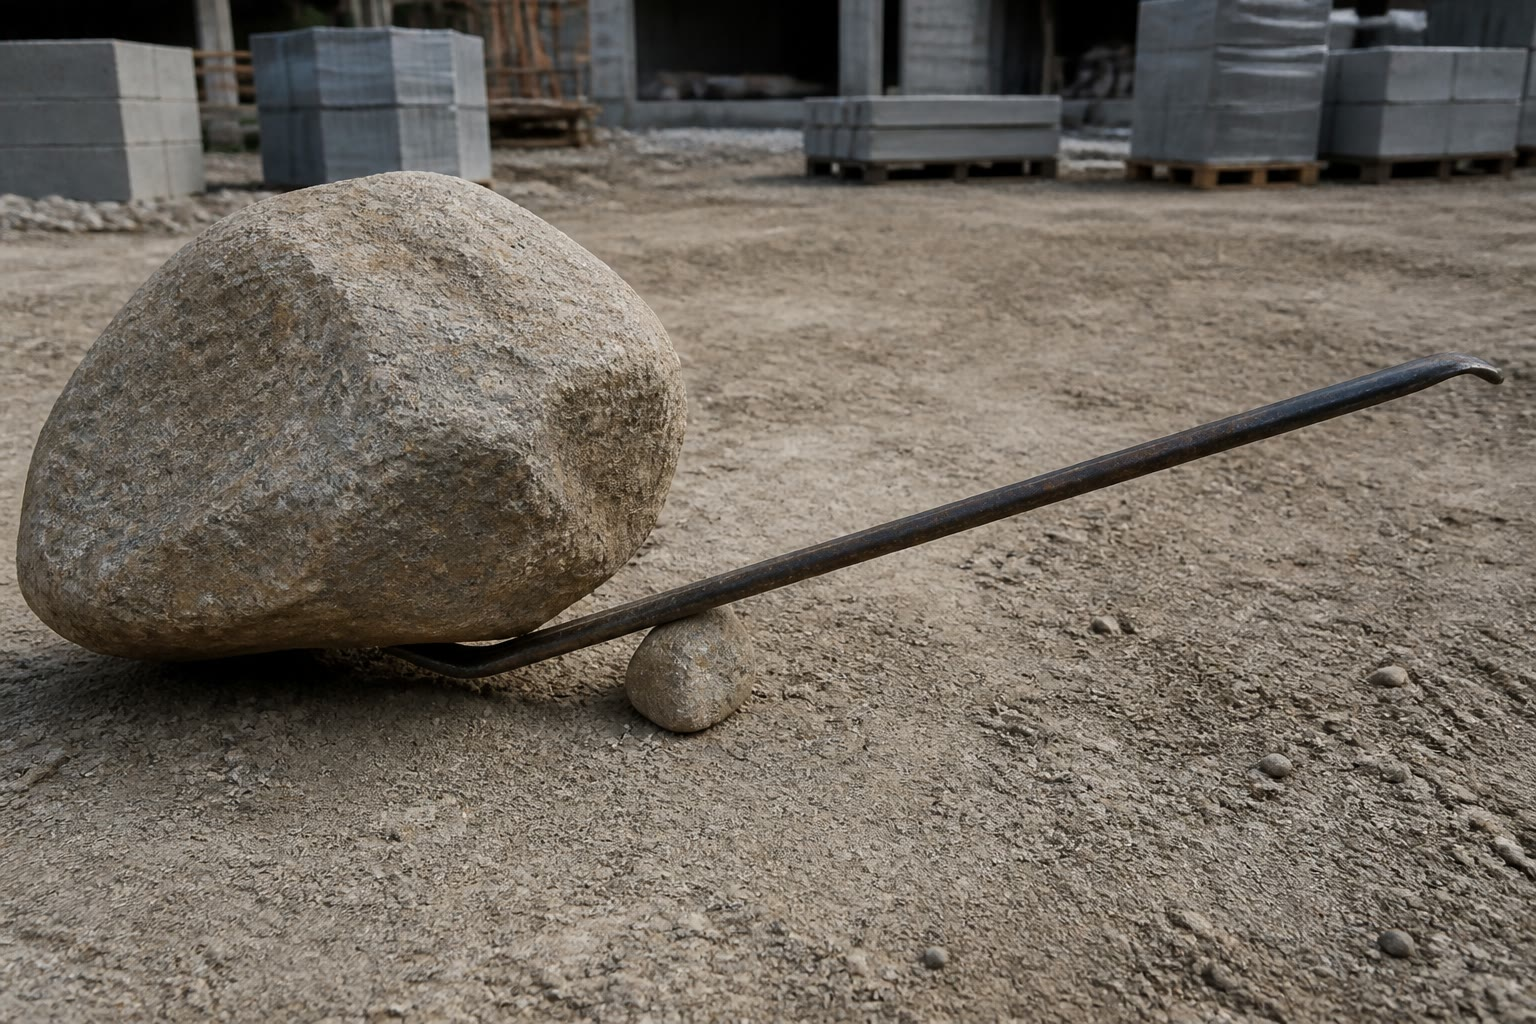
\includegraphics[width=0.55\linewidth]{images/book1/ai/g3-levers-crowbar.jpg}

{\small العتلة في عملها: دفعة صغيرة بعيدة عن \omterm{def:g3:levers-and-scales:lever}{محور الارتكاز} ترفع صخرة لا تحرّكها يد.}
\end{omfigure}

\section{قاعدة الرافعة}

\begin{method}[أرجوحة القطع النقدية]\label{met:g3:levers-and-scales:coins}
ابنِ أرجوحة متأرجحة مصغّرة لتصطاد القاعدة:
\begin{enumerate}
  \item وازِن مسطرة على قلم عند علامة منتصفها؛
  \item واستعمل قطعًا نقدية متماثلة ركّابًا، توضع عند علامات
        صحيحة: فقولنا ``قطعة عند $4$'' يعني أربع علامات من
        القلم؛
  \item حمّل الجانبين ولاحظ متى تتوازن المسطرة.
\end{enumerate}
جرّب: قطعة عند $6$ توازن قطعة عند $6$. وقطعتان مكدّستان عند $3$
توازنان قطعة عند $6$. وثلاث قطع عند $2$ --- توازن هي أيضًا واحدة
عند $6$!
\end{method}

\begin{proposition}[قاعدة الرافعة]\label{prop:g3:levers-and-scales:rule}
اضرب في كل جانب من \omterm{def:g3:levers-and-scales:lever}{الرافعة} عددَ القطع في بُعدها عن \omterm{def:g3:levers-and-scales:lever}{محور الارتكاز}.
وتتوازن \omterm{def:g3:levers-and-scales:lever}{الرافعة} تمامًا حين يكون للجانبين \emph{الجداء نفسه}:
\[
2 \text{ قطعة} \times 3 \text{ علامات} = 6
\qquad\text{توازن}\qquad
1 \text{ قطعة} \times 6 \text{ علامات} = 6 .
\]
وإن كان جداء أحد الجانبين أكبر نزل ذلك الجانب.
\end{proposition}

\begin{omfigure}
\begin{tikzpicture}[scale=0.85]
  \draw[thick, fill=omExo, fill opacity=0.3]
    (5.5,0) -- (5.9,0.7) -- (5.1,0.7) -- cycle;
  \draw[very thick] (1.0,0.78) -- (10.0,0.78);
  \foreach \x in {1.75,2.5,3.25,4.0,4.75,6.25,7.0,7.75,8.5,9.25} {
    \draw (\x,0.7) -- (\x,0.86);
  }
  \draw[thick, fill=omDef, fill opacity=0.5] (3.25,1.09) circle (0.3);
  \draw[thick, fill=omDef, fill opacity=0.5] (3.25,1.69) circle (0.3);
  \node[above, font=\small] at (3.25,2.1) {$2$ قطعة عند $3$};
  \draw[thick, fill=omThm, fill opacity=0.5] (9.25,1.09) circle (0.3);
  \node[above, font=\small] at (9.25,1.5) {$1$ قطعة عند $6$};
  \node[below, font=\small] at (5.5,-0.25)
    {$2 \times 3 = 6$ على اليسار، و$1 \times 6 = 6$ على اليمين:
     توازن};
\end{tikzpicture}

{\small قاعدة \omterm{def:g3:levers-and-scales:lever}{الرافعة} على مسطرة: جداءان متساويان، وقضيب مستوٍ.}
\end{omfigure}

\begin{example}[استعمال القاعدة]\label{ex:g3:levers-and-scales:using}
أربع قطع عند العلامة $2$: جداؤها $4 \times 2 = 8$. ولموازنتها
بقطع عند العلامة $4$ نحتاج إلى جداء قدره $8$ هناك أيضًا:
$8 = 2 \times 4$، فتكفي قطعتان عند $4$. وهل تستطيع قطعة واحدة أن
توازن الأربع؟ عليها أن تجلس عند العلامة $8$: $1 \times 8 = 8$.
فكلما خفّ الراكب وجب أن يجلس أبعد --- وهو بعينه ما علّمتنا إياه
أرجوحة بابا، لكن بالأعداد الآن.
\end{example}

\section{ميزان الكفّتين}

\begin{definition}[ميزان الكفّتين]\label{def:g3:levers-and-scales:scale}
\emph{ميزان الكفّتين}\index{ميزان كفّتين} \omterm{def:g3:levers-and-scales:lever}{رافعة} مبنيّة للعدل:
كفّتان معلّقتان على بُعدين \emph{متساويين تمامًا} من \omterm{def:g3:levers-and-scales:lever}{محور
الارتكاز}. ومع تساوي البُعدين يتساوى الجداءان تمامًا حين يتساوى
الوزنان --- فيميل الميزان نحو الكفّة الأثقل، ويستوي حين تحمل
الكفّتان حِملين متساويي الثقل.
\end{definition}

\begin{omfigure}
\begin{tikzpicture}[scale=0.85]
  \draw[thick] (5.5,0) -- (5.5,2.6);
  \draw[thick] (4.9,0) -- (6.1,0);
  \draw[very thick] (2.5,2.6) -- (8.5,2.6);
  \fill (5.5,2.6) circle (2.4pt);
  \draw[thick] (2.5,2.6) -- (2.2,1.5) (2.5,2.6) -- (2.8,1.5);
  \draw[thick] (1.9,1.5) .. controls (2.5,1.05) .. (3.1,1.5);
  \draw[thick] (8.5,2.6) -- (8.2,1.5) (8.5,2.6) -- (8.8,1.5);
  \draw[thick] (7.9,1.5) .. controls (8.5,1.05) .. (9.1,1.5);
  \fill[omDef, opacity=0.5] (2.5,1.5) circle (0.28);
  \fill[omThm, opacity=0.5] (8.35,1.42) circle (0.22);
  \fill[omThm, opacity=0.5] (8.68,1.42) circle (0.22);
  \node[below, font=\small] at (5.5,-0.3)
    {ذراعان متساويان: فيقارن الميزان الكفّتين بعدل};
\end{tikzpicture}

{\small \omterm{def:g3:levers-and-scales:scale}{ميزان الكفّتين}: \omterm{def:g3:levers-and-scales:lever}{رافعة} بكفّتين على بُعدين متساويين.
واستواء الكفّتين يعني حِملين متساويي الثقل.}
\end{omfigure}

\begin{example}[الوزن بالمقارنة]\label{ex:g3:levers-and-scales:weighing}
باع التجّار آلاف السنين الطحين والذهب والفلفل بموازين الكفّتين:
السلعة في كفّة، وقطع معدنية مرجعية صغيرة في الأخرى، ويضيفون القطع
حتى تستوي الكفّتان. والميزان لا يعرف أعدادًا --- إنما يجيب
``أثقل'' أو ``أخفّ'' أو ``متساويان''. لكن المقارنة بقطع مختارة
جيدًا كل ما تحتاج إليه سوق عادلة --- وهي، كما سيبيّن آخر فصل من
هذا الجزء، الطريق إلى \omterm{def:g2:measuring-length:measure}{قياس} الكتلة نفسها.
\end{example}

\begin{remark}[افحص الميزان فارغًا]\label{rem:g3:levers-and-scales:fair}
الميزان العادل يجب أن يستوي وهو \emph{فارغ}. فإن كان أحد ذراعيه
أطول أو إحدى كفّتيه أثقل اختلف الجداءان قبل أن تصل السلعة أصلًا،
وغشّ كل وزن بعد ذلك. وكان التجّار الأمناء يثبتون استواء ميزانهم
الفارغ أمام الزبون --- وهي طريقة قديمة صامتة لقول ``لعب نظيف''.
\end{remark}

\section{تمارين}

\begin{exercise}[$\star$]\label{exo:g3:levers-and-scales:1}
عيّن \omterm{def:g3:levers-and-scales:lever}{الرافعة} \omterm{def:g3:levers-and-scales:lever}{ومحور الارتكاز} في: أرجوحة متأرجحة؛ \ عتلة على جذع؛
\ مقصّ. (والمقصّ يخبّئ رافعتين --- فأين يرتكزان؟)
\end{exercise}

\begin{exercise}[$\star$]\label{exo:g3:levers-and-scales:2}
لرفع صخرة ثقيلة بعتلة، أتضغط قريبًا من \omterm{def:g3:levers-and-scales:lever}{محور الارتكاز} أم بعيدًا
عنه؟ ولماذا، في جملة واحدة؟
\end{exercise}

\begin{exercise}[$\star$]\label{exo:g3:levers-and-scales:3}
على أرجوحة القطع النقدية، احسب الجداء في: $3$ قطع عند العلامة
$4$؛ \ $2$ قطعة عند العلامة $5$؛ \ $1$ قطعة عند العلامة $6$. وأيّ
زوج منها يوازن الآخر؟
\end{exercise}

\begin{exercise}[$\star$]\label{exo:g3:levers-and-scales:4}
قطعة واحدة عند العلامة $8$ على اليسار. فأين تضع $2$ من القطع على
اليمين لتوازنها؟ وأين تضع $4$ قطع؟
\end{exercise}

\begin{exercise}[$\star$]\label{exo:g3:levers-and-scales:5}
الجانب الأيسر: $3$ قطع عند العلامة $3$. والجانب الأيمن: $2$ قطعة
عند العلامة $4$. احسب الجداءين. وأيّ الجانبين ينزل؟
\end{exercise}

\begin{exercise}[$\star$]\label{exo:g3:levers-and-scales:6}
لماذا تُعلَّق كفّتا \omterm{def:g3:levers-and-scales:scale}{ميزان الكفّتين} على بُعدين متساويين تمامًا من
\omterm{def:g3:levers-and-scales:lever}{محور الارتكاز}؟ وماذا يفعل ذراع أيسر أطول بكل عملية وزن؟
\end{exercise}

\begin{exercise}[$\star$]\label{exo:g3:levers-and-scales:7}
يستوي \omterm{def:g3:levers-and-scales:scale}{ميزان كفّتين} وفي إحدى كفّتيه كيس كرات زجاجية وفي الأخرى
$6$ قطع متماثلة. فماذا نعلم عن الكيس؟ وبماذا يجيب الميزان إن
نزعنا قطعة واحدة؟
\end{exercise}

\begin{exercise}[$\star$]\label{exo:g3:levers-and-scales:8}
أرجوحة متأرجحة: يزن توم قدر $2$ من الأكياس ويجلس عند العلامة
$3$؛ وتزن أخته الصغيرة قدر كيس واحد. فعند أيّ علامة يجب أن تجلس
لتوازنه؟
\end{exercise}

\begin{exercise}[$\star$]\label{exo:g3:levers-and-scales:9}
مخلب المطرقة ينزع مسمارًا: يدك تدفع طرف المقبض، بعيدًا عن الموضع
الذي يستند فيه رأس المطرقة إلى الخشب. فأيّ الموضعين \omterm{def:g3:levers-and-scales:lever}{محور
الارتكاز}، ولماذا يخرج المسمار الذي لم تكن أصابعك لتنزعه أبدًا؟
\end{exercise}

\begin{exercise}[$\star\star$]\label{exo:g3:levers-and-scales:10}
يريد الجدّ (وثقله $4$ أكياس) أن يتأرجح مع زوي الصغيرة (وثقلها
كيس واحد). وعلى الأرجوحة علامات من $1$ إلى $8$ في كل جانب. جِد
\emph{طريقتين} مختلفتين لإجلاسهما بحيث تتوازن الأرجوحة.
\end{exercise}

\begin{exercise}[$\star\star$]\label{exo:g3:levers-and-scales:11}
تاجر غشّاش يجعل أحد ذراعَي ميزانه أطول قليلًا في الخفاء، ويضع
السلعة دائمًا في جهة الذراع الطويل. أينال الزبائن سلعة أكثر ممّا
يدفعون أم أقلّ؟ اشرح بقاعدة \omterm{def:g3:levers-and-scales:lever}{الرافعة} --- وبما في
\cref{rem:g3:levers-and-scales:fair}.
\end{exercise}
